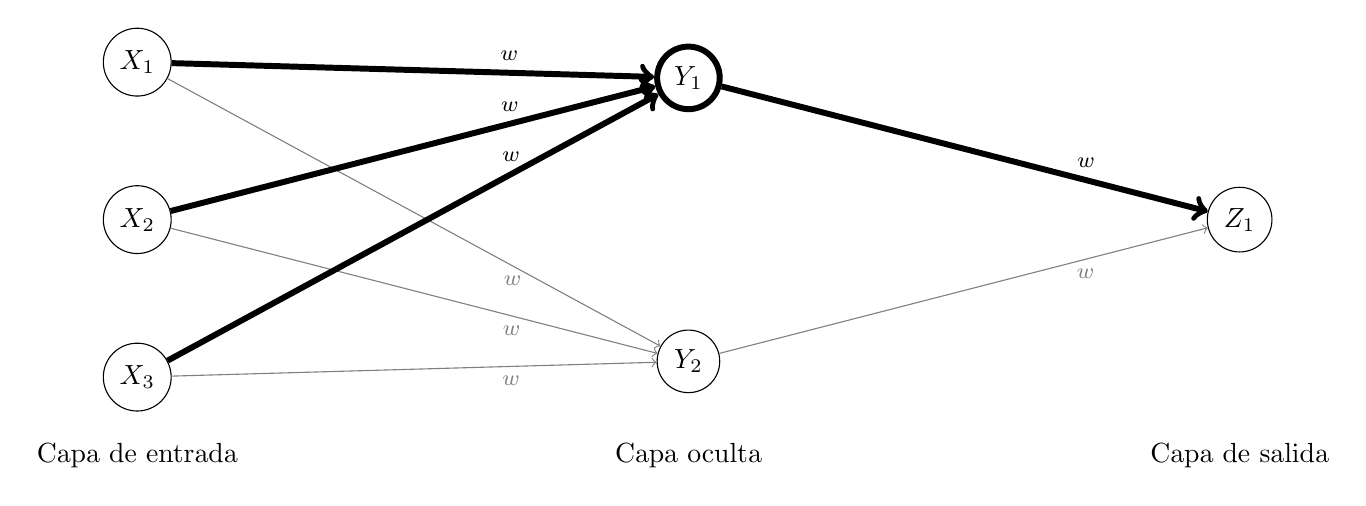
\begin{tikzpicture}

	\tikzstyle{nodo}=[circle, draw, minimum size=5ex]
	\tikzstyle{upw}=[dashed, red, ->, line width = 1pt]
	\tikzstyle{bold}=[line width=0.5ex]

	\coordinate (l_0) at (0, 3.5);
	\coordinate (l_1) at (7, 3.5);
	\coordinate (l_2) at (14, 3.5);
	\coordinate (input) at (0, -3.0);
	\coordinate (hidden) at (7, -3.0);
	\coordinate (output) at (14, -3.0);

	\coordinate (f_1_1) at (0, 2.0); % CAPA ENTRADA
	\coordinate (f_1_2) at (0, 0); % CAPA ENTRADA
	\coordinate (f_1_3) at (0, -2.0); % CAPA ENTRADA
	\coordinate (f_2_1) at (7, 1.8); % CAPA OCULTA 1
	\coordinate (f_2_2) at (7, -1.8); % CAPA OCULTA 1
	\coordinate (f_3_1) at (14, 0); % CAPA SALIDA

	%\node[] (l_0) at (l_0) {$L - 1$};
	%\node[] (l_1) at (l_1) {$L$};
	%\node[] (l_2) at (l_2) {$L + 1$};
	\node[] (input) at (input) {Capa de entrada};
	\node[] (hidden) at (hidden) {Capa oculta};
	\node[] (output) at (output) {Capa de salida};

	\node[nodo] (f_1_1) at (f_1_1) { $X_1$}; % CAPA ENTRADA
	\node[nodo] (f_1_2) at (f_1_2) { $X_2$}; % CAPA ENTRADA
	%\node[nodo] (f_1_3) at (f_1_3) {\Large $f_i(e_i)$}; % CAPA ENTRADA
	\node[nodo] (f_1_3) at (f_1_3) { $X_3$}; % CAPA ENTRADA
	\node[nodo, bold] (f_2_1) at (f_2_1) { $Y_1$}; % CAPA OCULTA 1
	\node[nodo] (f_2_2) at (f_2_2) { $Y_2$}; % CAPA OCULTA 1
	\node[nodo] (f_3_1) at (f_3_1) { $Z_1$}; % CAPA SALIDA


	\draw[->, font=\footnotesize, gray] (f_1_1) -- node[pos=0.70, below] (w_2_1) {$w$} (f_2_2);
	\draw[->, font=\footnotesize, gray] (f_1_2) -- node[pos=0.70, below] (w_2_2) {$w$} (f_2_2);
	\draw[->, font=\footnotesize, gray] (f_1_3) -- node[pos=0.70, below] (w_2_3) {$w$} (f_2_2);
	\draw[->, font=\footnotesize, bold] (f_1_1) --  node[pos=0.7, above] (w_1_1) {$w$} (f_2_1);
	\draw[->, font=\footnotesize, bold] (f_1_2) --  node[pos=0.70, above] (w_1_2) {$w$} (f_2_1);
	\draw[->, font=\footnotesize, bold] (f_1_3) -- node[pos=0.70, above] (w_1_3) {$w$} (f_2_1);

	\draw[->, font=\footnotesize, gray] (f_2_2) -- node[near end, below] {$w$} (f_3_1);
	\draw[->, font=\footnotesize, bold] (f_2_1) -- node[near end, above ] (w_j_k) {$w$} (f_3_1);
\end{tikzpicture}
